
\chapter{The complete plane: additional components}
\section{High lift devices}	
	The main objective of lift is to counterbalance the weight: 
	
	\begin{equation}
	W = L = C_L \frac{1}{2} \rho _\infty V_\infty ^2 S.
	\end{equation}
	
	Suppose now that $V_\infty \ll$, there are 2 options to increase lift: increasing $C_L$ or increasing $S$. The problem is that the 2 solutions increase the drag, the first need an increased camber, and for the second $D = C_D \frac{1}{2} \rho _\infty V_\infty ^2 S$. The best solution is to increase $C_L$ only for $V_\infty \ll$ and this can be done by changing the geometry or by controlling the boundary layer (attached flow). 
	
\subsection{Trailing edge flaps}
\subsubsection{Plain flap}
	\wrapfig{4}{r}{5}{0.1}{ch5/1}{ch5/1}
	The principle of flaps is to increase the camber. This is the most simple, the trailing edge shifts downward, increasing $C_L$. The characteristics are: 
	\begin{itemize}
	\item[•] Because of separation appearing earlier $\alpha _{stall} \searrow$, this is better for the view of the pilot. 
	\item[•] $C_L(max)$ is up to 50\% higher, reached for high deflection $\approx 80\degres$.
	\item[•] The drag increases much more than the lift $C_L/C_D \searrow$, this is good for landing as it helps to decelerate.
	\item[•] Center of pressure at the trailing edge $\rightarrow \Delta C_m<0$ (nose down). 
	\end{itemize}
	
\subsubsection{Split flap}
	\wrapfig{3}{r}{3}{0.15}{ch5/2}{ch5/2} \ \\
	\begin{itemize}
	\item[•] Separation appears later than the previous case, $\alpha _{stall} \searrow$ less. 
	\item[•] Larger wake because of the split $\rightarrow$ more drag, not good for take off. 
	\item[•] $C_L(max) \nearrow$ up to 60\% and nose down less than previous case. 
	\end{itemize}
	
\subsubsection{Slotted flap}
	\wrapfig{5}{l}{4}{0.1}{ch5/3}{ch5/3}
	In this case $\alpha _{stall}$ increases compared to plain because of the slot allowing the control of separation and the increase of $C_D$ is smaller than the plain flap. $C_L(max) \approx 65\%$.
	
	\ \\
	
\subsubsection{Fowler flap}
	\wrapfig{6}{r}{4}{0.1}{ch5/4}{ch5/4}
	This the most used type of flap, combination of the slotted flap and a backward motion: 
	
	\begin{itemize}
	\item[•] $C_L \nearrow$ further compared to slotted.  
	\item[•] $\alpha _{stall} \searrow$ compared to slotted because of $\frac{t}
{c}\searrow$.
	\item[•] $\Delta C_D \searrow$ because boundary layer control + $\frac{t}{c} \searrow$.
	\item[•] $\Delta C_m \gg$ because flap going backward. In practice, the fowler flap contains many slots. 
	\end{itemize}
	
	The figures below shows a good summary. 
	
	\begin{center}
	\begin{minipage}{0.25\textwidth}
	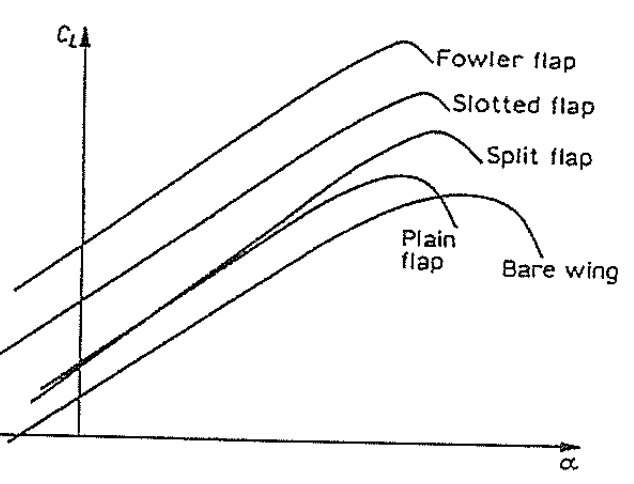
\includegraphics[scale=0.15]{ch5/5}
	\captionof{figure}{}	
	\end{minipage}
	\begin{minipage}{0.25\textwidth}
	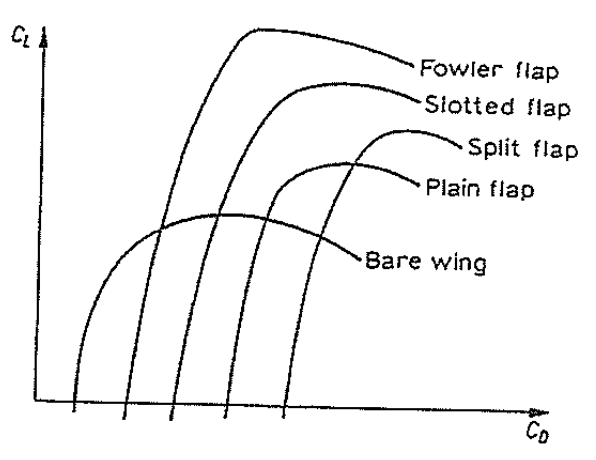
\includegraphics[scale=0.15]{ch5/6}
	\captionof{figure}{}	
	\end{minipage}
	\begin{minipage}{0.3\textwidth}
	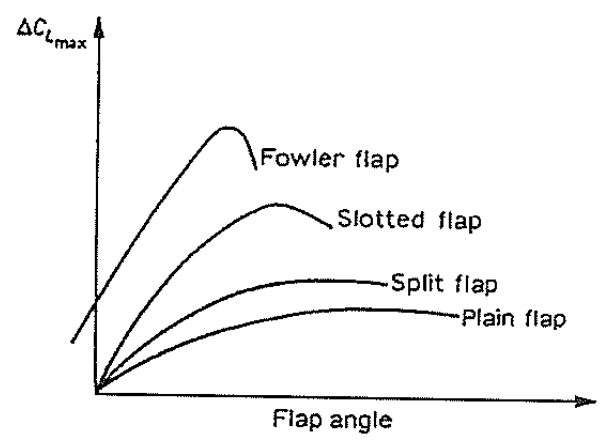
\includegraphics[scale=0.2]{ch5/7}
	\captionof{figure}{}	
	\end{minipage}
	\end{center}
	
\paragraph{Remarks}
	\begin{itemize}
	\item[•] $\frac{dC_m}{dC_L}\approx cst$, this implies that k in $C_m = C_{m0} + k C_L$ does not change and that the \textbf{aerodynamic center} doesn't change. 
	
	\item[•] The flaps are placed near the fuselage, this decreases the efficiency, changes the loft distribution on the wing that have effect on $D_i$ and the pressure center closer to the fuselage can have effects on the stability. 
	
	\item[•] Other types of flaps: Zap flap (split + fowler), $C_L$ is higher than the split but the drag is higher than fowler. 
	\end{itemize}		
	
\subsection{Slat}
	\minifig{ch5/8}{ch5/9}{0.2}{0.15}{0.3}{0.3}
	The slats are separated from the airfoil by a slot. This allows to energies the boundary layer by a flow through the slot. This has no effect for small $/alpha$, it allows to increase $\alpha _{stall}$ going from 15\degres to 25\degres, increasing $C_L(max)$ up to 60\%. The disadvantage is that for low speeds the drag decreases (less detached boundary), this is bad for landing. And for higher speeds the flow disturbance increases the drag. \textbf{Controllable slats} are necessary. \\
	
	The second disadvantage is that to have the lift increase effect we nee to go to very high $\alpha$, not good for the sight of the pilot. 
	
\subsection{Leading edge flap}
	\minifig{ch5/10}{ch5/11}{0.2}{0.2}{0.3}{0.3}
	Deflection at high $\alpha$ can prevent LE separation, and this even more for high velocity wings with sharp LE. The lift coefficient increases because of increased camber, but the $\alpha _{stall}$ is less than the slat. Indeed all of these are used together nowadays. 
	
\section{Boundary layer control}	
\paragraph{Boundary layer blowing}
	We saw previously that it was possible to energize the boundary layer by injecting high speed air throw slots. This makes increase $\alpha _{stall}$ and the high velocity increases the circulation, thus $L \ \forall \alpha$. 
	
\paragraph{Boundary layer suction}
	This consist in sucking away the low velocity air by means of porous wings or suction holes. 
	
\paragraph{Remark}
	\wrapfig{6}{l}{5}{0.15}{ch5/12}{ch5/12}
	For vertical or short take off and landing, the engine jet is used. The air coming from the engine is redirected to energize the boundary layer. VTOL: jet engine is deflected vertically for vertical take off, where the thrust must be equal to the weight, while it is about 30\% for horizontal take off. 
	
\section{Tailplanes}
	\wrapfig{6}{r}{3.5}{0.15}{ch5/13}{ch5/13}
	Consider $\alpha$ small so that the lift is assumed perpendicular to the chord, applied on the AC and the weight is applied on the center of gravity. The moment in the center of gravity is:
	
	\begin{equation}
	C_m = C_{M_0} + C_L (h-h_0) \qquad \Rightarrow \frac{dC_m}{dC_L} = h -h_0 > 0.
\end{equation}	 

	And since $dC_L/d\alpha = m$:
	
	\begin{equation}
	\frac{dC_m}{d\alpha} = m(h-h_0)>0
	\end{equation}
	
	\wrapfig{5}{r}{5}{0.15}{ch5/14}{ch5/14}
	and the wing is \textbf{statically unstable} because the increase in $\alpha$ causes an increase in $C_m$ and so even more nose up. We see that in fact the wing alone is stable only if the center of gravity is upstream of the aerodynamic center. 
	\textbf{Tail} planes are used to increase stability, one has now: 
	
	\wrapfig{6}{l}{3}{0.15}{ch5/15}{ch5/15}
	\begin{equation}
	\frac{dC_m}{d\alpha} = m(h-h_0) - \frac{C_{L_T}}{d\alpha} \gamma 
	\end{equation}
	
	where $\gamma = \frac{l S_T}{cS}$ as $C_{L_T} = \frac{L_T}{0.5\rho _\infty V_\infty ^2 S_T}$. One can reach stability for sufficiently high $\gamma$, by increasing $l$ or $S_T$. 
	
	An alternative to tail planes are the \textbf{cannards} as illustrated here. 